!TeX root = BasiDiDati.tex
 
 \chapter{Strutture fisiche e di accesso ai dati}
  Le basi di dati risiedono nella \textcolor{azzurrino}{\textbf{memoria secondaria}} perchè sono:
  \begin{itemize}[label=$\triangleright$]
    \item \textbf{grandi}: non possono essere contenute completamente in memoria centrale
    \smallskip
    \item \textbf{persistenti}: hanno un tempo di vita che non è limitato all'esecuizone dei programmi che le usano
  \end{itemize}

  \vario{Caratteristiche della memoria secondaria}{
    Le caratteristiche principali della memoria secondaria sono:
    \begin{itemize}[label=$\circ$]
      \item non utilizzabile direttamente dai programmi
      \smallskip
      \item dati organizzati in \textbf{blocchi} (grandezza dipende dal sistema operativo)
      \smallskip
      \item operazioni possibili:
      \begin{itemize}[label=$\diamond$]
        \item lettura intero blocco
        \item scrittura intero blocco
      \end{itemize}
      \smallskip
      \item costo delle operazioni di accesso alla memoria secondaria è maggiore al costo per accedere ai dati in memoria centrale
    \end{itemize}
  }

  \section{Gestore del buffer}
  L'interazione tra memoria secondaria e memoria centrale avviene tramite il \textcolor{azzurrino}{\textbf{gestore del buffer}} tramite il trasferimento di uno o più \textbf{blocchi} della memoria secondaria in \textbf{pagine} dedicate della memoria centrale (buffer).

  \vario{Precisazione}{
    La dimensione delle pagine in memoria centrale sono siltamente un multiplo della dimensione dei blocchi in memoria secondaria.

    \smallskip
    Per semplificare, si assume che siano uguali:
    \begin{equation*}
      \text{1 pagina} \approx \text{1 blocco}
    \end{equation*}
  }

  \subsection{Buffer}
  Il \textcolor{azzurrino}{\textbf{buffer}} è una zona della memoria condivisa dalle applicazioni e una gestiona ottimale del buffer consente di ottenere buone prestazioni nell'accesso ai dati.\\[0.2ex]
  Quando uno stesso dato viene utilizzato più volte in tempi ravvicinati il buffer evita
  l’accesso alla memoria secondaria.

  \vario{Compito del gestore del buffer}{
    Il gestore del buffer si occupa del caricare e salvare i dati dalla memoria secondaria alla memoria centrale.
  }

  \subsection{Politica di gestione della memoria}
  L'obiettivo del gestore del buffer è di \hl{ottimizzare gli accessi} attraverso le politiche di gestione della memoria:
  \begin{itemize}[label=$\diamond$]
    \item \textbf{lettura di un blocco}:
    \begin{itemize}[label=$\triangleright$]
      \item blocco presente in una pagina del buffer
      \begin{itemize}[label=$\Rightarrow$]
        \item non viene eseguita la lettura in memoria secondaria
        \smallskip
        \item viene restituito un puntatore alla pagine del buffer
      \end{itemize}
      \medskip
      \item blocco non presente in una pagina del buffer
      \begin{itemize}[label=$\Rightarrow$]
        \item viene cercata una pagina libera
        \smallskip
        \item viene caricato il blocco nella pagina
        \smallskip
        \item viene restituito il puntatore alla pagina del buffer
      \end{itemize}
    \end{itemize}
    \bigskip
    \item \textbf{scrittura di un blocco}: se viene effettuata una richiesta si dcrittura di un blocco giù caricato in una pagina del buffer, il gestore del buffer può decidere di \hl{differire la scrittura} su memoria secondaria in un secondo momento
  \end{itemize}

  \medskip
  Per poter aumentare la velocità di accesso ai dati, le politiche di lettura e scrittura si basano sul \textbf{principio di località}.

  \definizione{principio di località}{
    Il \textbf{principio di località} si basa sul fatto che i dati refernziati di recente hanno maggiore probabilità di essere referenziati nuovamente in futuro.
  }

  \subsection{Gestione delle pagine}
  Il contenuto del buffer lo possiamo immaginare come una matrice.

  \begin{figure}[H]
    \centering
    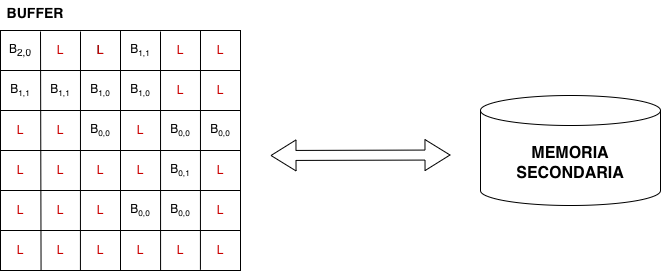
\includegraphics[width=0.5\textwidth]{images/gestione-pagine.png}
  \end{figure}

  Per ogni pagina del buffer si memorizza:
  \begin{itemize}[label=$\triangleright$]
    \item blocco B (L se libero) indicando il file e il numero di blocco (offset)
    \smallskip
    \item variabili di stato ($B_{i,j}$):
    \begin{itemize}[label=$\circ$]
      \item contatore i: indica il numero di transazioni
      \item bit di stato j: indica se la pagina è stata modificata (1) o no (0)
    \end{itemize}
  \end{itemize}

  \subsection{Primitive per la gestione del buffer}

  \subsubsection{Primitiva \protect\texttt{fix}}
  La \textcolor{azzurrino}{primitiva \texttt{fix}} viene utilizzata dalle transazioni per richiedere l'accesso ad un blocco e restituisce un puntatore alla pagina contente il blocco richiesto.

  Le azioni della primitiva sono:
  \begin{itemize}[label=$\triangleright$]
    \item \textbf{ricerca del blocco}:
    \begin{itemize}[label=$\diamond$]
      \item blocco viene trovato
      \begin{itemize}[label=$\Rightarrow$]
        \item viene restituito un puntatore alla pagina contentente il blocco
      \end{itemize}
      \medskip
      \item blocco non viene trovato:
      \begin{itemize}[label=$\circ$]
        \item viene scelta una pagina libera
        \begin{itemize}[label=$\Rightarrow$]
          \item viene salvata in memoria secondaria (primitiva $\verb|flush|$)
          \item viene caricato il blocco in P aggiornando file e numero di blocco
        \end{itemize}
        \smallskip
        \item non ci sono pagine libere
        \begin{itemize}[label=$\Rightarrow$]
          \item viene rubata una pagina a un'altra transazione (primitiva $\verb|flush|$)
          \item viene sospesa la transazione inserendola in una cosa di attesa
          \item se si libera una pagina il gestore si comporterà come al punto precedente
        \end{itemize}
      \end{itemize}
    \end{itemize}
  \end{itemize}

  \medskip
  \begin{itemize}[label=$\Rightarrow$]
    \item \textbf{effetto della modifica}: quando una transizione accede a una pagina per la prima volta il contatore si incrementa
  \end{itemize}

  \subsubsection{Primitiva \protect\texttt{unfix}}
  La \textcolor{azzurrino}{primitiva \texttt{unfix}} viene usata dalle transazioni per indicare che la transazione ha terminato di usare il blocco.

  \begin{itemize}[label=$\Rightarrow$]
    \item \textbf{effetto della modifica}: decremento del contatore i
  \end{itemize}

  \subsubsection{Primitiva \protect\texttt{setDirty}}
  La \textcolor{azzurrino}{primitiva \texttt{setDirty}} viene utilizzata dalle transazioni per indicare al gestore del buffer che il blocco della pagina è stato modificato.

  \begin{itemize}[label=$\Rightarrow$]
    \item \textbf{effetto della modifica}: bit di stato J passa da 0 a 1
  \end{itemize}

  \subsubsection{Primitiva \protect\texttt{force}}
  La \textcolor{azzurrino}{primitiva \texttt{force}} viene utilizzata per salvare in memoria secondaria in \hl{modo sincrono} il blocco contenuto nella pagina.\\[0.2ex]
  Questa primitiva viene usata dal gestore dell'affidabilità.

  \begin{itemize}[label=$\Rightarrow$]
    \item \textbf{effetto della modifica}: viene salvato in memoria secondaria il blocco e il bit di stato J posto a 0
  \end{itemize}

  \subsubsection{Primitiva \protect\texttt{flush}}
  La \textcolor{azzurrino}{primitiva \texttt{flush}} viene utilizzata per salvare i blocchi in memoria secondaria in \hl{modo asincrono}.\\[0.2ex]
  Questa primitiva viene usata dal gestore del buffer.

  \begin{itemize}[label=$\Rightarrow$]
    \item \textbf{effetto della modifica}: viene liberta la pagina "dirty" e il bit di stato J viene posto a 0
  \end{itemize}

  \section{Gestore dell'affidabilità}
  Il gestore del buffer differisce le operazioni di scrittura e questo potrebbe raprresentare un pericolo.\\[0.2ex]
  Il \textcolor{azzurrino}{\textbf{gestore dell'affibilità}} si occupa di garantire:
  \begin{itemize}[label=$\triangleright$]
    \item \textbf{atomicità}: transazioni non devono essere incomplete
    \smallskip
    \item \textbf{persistenza}: effetti di ciascuna transazione non conclusa con un commit devono essere mantenuti in modo permanente
  \end{itemize}

  \begin{figure}[H]
    \centering
    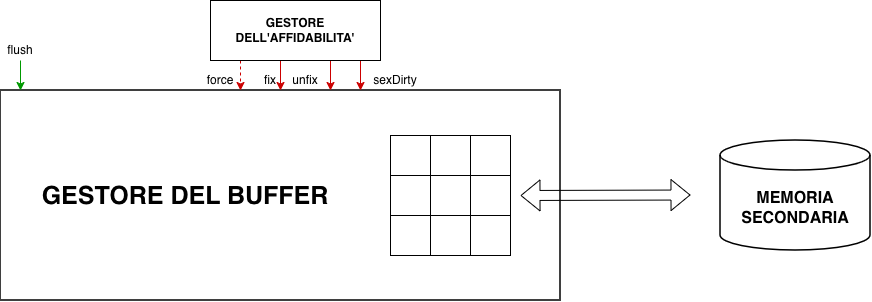
\includegraphics[width=0.6\textwidth]{images/gestore-affidabilità.png}
  \end{figure}


  \subsection{File di LOG}
  Il funzionamento del gestore dell'affidabilità si basa sull'utilizzo del \textbf{file di LOG}.

  \definizione{file di LOG}{
    Il \textbf{file di LOG} è un archivio persistente su cui vengono registrate tutte le operazioni eseguite dal DBMS.
  }

  Per il corretto funzionamento, il gestore dell’affidabilità deve disporre di un dispositivo di una \textbf{memoria stabile} (resistente ai guasti).

  Il file di LOG viene memorizzato in memoria stabile e al suo interno vengono memorizzati:
  \begin{itemize}[label=$\triangleright$]
    \item \textbf{record di transizione}: record che descrivono informazioni sulle transazioni
    \begin{itemize}[label=$\diamond$]
      \item $\boldsymbol{\mathrm{B(T)}}$: \textcolor{azzurrino}{\textbf{begin}} della transazione
      \smallskip
      \item $\boldsymbol{\textbf{C(T)}}$: \textcolor{azzurrino}{\textbf{commit}} della transazione
      \smallskip
      \item $\boldsymbol{\textbf{A(T)}}$: \textcolor{azzurrino}{\textbf{abort}} della transazione
      \smallskip
      \item $\boldsymbol{\textbf{I(T,O,AS)}}$: \textcolor{azzurrino}{\textbf{insert}} di un oggetto da parte di una transazione $\mathrm{T}$ con il suo after state $\mathrm{AS}$ (stato dell'oggetto dopo l'operazione)
      \smallskip
      \item $\boldsymbol{\mathrm{D(T,O,BS)}}$: \textcolor{azzurrino}{\textbf{delete}} di un oggetto $\mathrm{O}$ da parte della transizione $\mathrm{T}$ con il suo before state $\mathrm{BS}$ (stato dell'oggetto prima dell'operazione)
      \smallskip
      \item $\boldsymbol{\mathrm{U(T,O,BS,AS)}}$: \textcolor{azzurrino}{\textbf{update}} di un oggetto $\mathrm{O}$ da parte della transizione $\mathrm{T}$ con il suo before state $\mathrm{BS}$ e il suo after state $\mathrm{AS}$
    \end{itemize}
    \medskip
    \item \textbf{record di sistema}: record che descrivono informazioni sulle operazioni esaguite dal DBMS
    \begin{itemize}[label=$\circ$]
      \item $\boldsymbol{\mathrm{DUMP}}$: copia completa e consistente della base di dati.
      \smallskip
      \item $\boldsymbol{\mathrm{CK}(T_1, \dots, T_n)}$: indica che all'esecuzione del checkpoint, le transazioni attive erano $T_1, \dots, T_n$
      \begin{itemize}
        \item elenco delle transazioni che non hanno ancora espresso la loro scelta relativamente all'esito finale
        \smallskip
        \item operazione svolta periodicamente affinché i dati delle transazioni che hanno eseguito il \texttt{commit} siano registrati in modo permanente
        \smallskip
        \item il protocollo di checkpoint prevede i seguenti passi:
        \begin{enumerate}
          \item sospensione delle operazioni di scrittura, \texttt{commit} e \texttt{abort} delle transazioni
          \smallskip
          \item esecuzione della primitiva \texttt{force} sulle pagine ``dirty'' di transazioni che hanno eseguito il \texttt{commit}
          \smallskip
          \item scrittura sincrona (primitiva \texttt{force}) sul file di LOG del record di checkpoint con gli identificatori delle transazioni attive
          \smallskip
          \item ripresa delle operazioni di scrittura, \texttt{commit} e \texttt{abort} delle transazioni
        \end{enumerate}
      \end{itemize}
    \end{itemize}
  \end{itemize}

I record di transazione salvati nel LOG consentono di eseguire in caso di ripristino le seguenti operazioni:
\begin{itemize}[label=$\triangleright$]
  \item $\boldsymbol{\mathrm{UNDO}}$: viene usato per disfare un'azione su un oggetto $\mathrm{O}$ è sufficiente ricopiare in $\mathrm{O}$ il valore d $\mathrm{BS}$.
  
  L'insert/delet viene disfatto cancellando/inserendo $\mathrm{O}$
  \smallskip
  \item $\boldsymbol{\mathrm{REDO}}$: serve per rifare un'azione su un oggetto $\mathrm{O}$ è sufficiente ricopiare in $\mathrm{O}$ il valore $\mathrm{AS}$.
  
  L'insert/delete viene rifatto inserendo/cancellando $\mathrm{O}$
\end{itemize}

\medskip
Gli inserimenti controllano sempre l’esistenza di $\mathrm{O}$ prima di eseguire l'operazione.\\[0.2ex]
Per queste operazioni vale la \textbf{proprietà di idempotenza}.

\definizione{proprietà di idempotenza}{
  \[
    \begin{aligned}
      \mathrm{UNDO(UNDO(A))} &= \mathrm{UNDO(A)}\\
      \mathrm{REDO(REDO(A))} &= \mathrm{REDO(A)}
    \end{aligned}
  \]
}

\subsection{Regole di scrittura sul file di log}
Il gestore dell'affibilità deve rispettare le seguenti regole di scrittura sul file di LOG:
\begin{itemize}[label=$\Rightarrow$]
  \item \textbf{regola Write Ahead Logging}:record di LOG devono essere scritti sul LOG precedente all'esecuzione delle corrispondenti operazioni sulla base di dati (garantisce la possibilità di fare sempre UNDO)
  \smallskip
  \item \textbf{regola di commit-precedenza}: record di LOG devono essere scritti sul LOG prima dell'esecuzione del $\texttt{commit}$ della transazione (garantisce la possibilità di fare sempre REDO)
\end{itemize}

 Queste regole consentono di salvare i blocchi delle pagine “dirty” in modo totalmente asincrono rispetto al commit delle transazioni.

\subsection{Guasti}
Una transazione T sceglie in modo atomico l’esito di $\verb|commit|$ nel momento in cui
scrive nel file di log in modo sincrono (primitiva $\verb|force|$) il suo record di $\verb|commit| \ \mathrm{C(T)}$. 

\begin{itemize}[label=$\Rightarrow$]
  \item se avviene un guasto prima della scrittura del record di $\verb|commit|$ $\rightarrow$ $\boldsymbol{\mathrm{UNDO}}$
  \smallskip
  \item se avviene un guasto dopo la scrittura del record di $\verb|commit|$ $\rightarrow$ $\boldsymbol{\mathrm{REDO}}$
\end{itemize}

Esistono due tipologie di guasto:
\begin{itemize}[label=$\triangleright$]
  \item \textbf{guasto di sistema}: perdita del conte della memoria centrale.
  
  Viene risolto con la tecnica della \hl{ripresa a caldo}:
  \begin{enumerate}
    \item accede al file di LOG e si ripercorre all’indietro il LOG fino al più recente record di checkpoint
    \smallskip
    \item si inizializza:
    \begin{itemize}[label=$\diamond$]
      \item insieme $\mathrm{UNDO}$ con tutte le transazioni da disfare (presenti nel checkpoint)
      \smallskip
      \item insieme $\mathrm{REDO}$ con tutte le transazioni da rifare ($\emptyset$)
    \end{itemize}
    \smallskip
    \item si ripercorre in avanti il LOG
    \begin{itemize}[label=$\circ$]
      \item per ogni record $\mathrm{B(T)}$ incontrato si aggiunge T all’insieme $\mathrm{UNDO}$
      \smallskip
      \item per ogni record $\mathrm{C(T)}$ incontrato si sposta T dall’insieme $\mathrm{UNDO}$ all’insieme $\mathrm{REDO}$
    \end{itemize}
    \smallskip
    \item si ripercorre all’indietro il LOG disfacendo le operazioni eseguite dalle transazioni $\mathrm{UNDO}$ risalendo fino alla prima azione della transazione più vecchia
    \item si ripercorre in avanti il LOG per rifare le operazioni eseguite dalle transazioni $\mathrm{REDO}$
  \end{enumerate}
  \medskip
  \item \textbf{guasto di dispositivo}: perdita di parte o tutto il contenuto della base di dati in memoria secondaria.
  
  Viene risolto con la tecninca della \hl{ripresa a freddo}:
  \begin{enumerate}
    \item si accede al $\mathrm{DUMP}$ della base di dati e si ricopia selettivamente la parte deteriorata della base di dati
    \smallskip
    \item si accede al LOG risalendo al record di $\mathrm{DUMP}$
    \smallskip
    \item si ripercorre in avanti il LOG rieseguendo tutte le operazioni relative alla perte deteriorata comprese le azioni di $\verb|commit|$ e $\verb|abort|$
    \smallskip
    \item si applica una ripresa a caldo
  \end{enumerate}
\end{itemize}

\esempio{file di LOG}{
  Consideriamo il seguente file di LOG:
  \[
    \begin{aligned}
      & \mathrm{B(T_1), B(T_2), U(T_2, O_1, B_1, A_1), I(T_1, O_2, A_2), B(T_3), C(T_1), B(T_4),} \\
      & \mathrm{U(T_3, O_2, B_3, A_3), U(T_4, O_3, B_4, A_4), CK(T_2, T_3, T_4), C(T_4), B(T_5),} \\
      & \mathrm{U(T_3, O_3, B_5, A_5), U(T_5, O_4, B_6, A_6), D(T_3, O_5, B_7), A(T_3), C(T_5),} \\
      & \mathrm{I(T_2, O_6, A_8)} \text{ \textbf{guasto}}
    \end{aligned}
  \] 

  \textcolor{red}{\textbf{Che passi svolge la ripresa a caldo?}}
  \begin{enumerate}
    \item risale il LOG fino all'ultimo record di checkpoint $\mathrm{CK(T_2,T_3,T_4)}$
    \smallskip
    \item inizializza $\mathrm{UNDO}$ e $\mathrm{REDO}$
    \begin{itemize}[label=$\triangleright$]
      \item $\mathrm{UNDO = \{T_2, T_3, T_4\}}$ (inizializzato con le transazioni del checkpoint)
      \smallskip
      \item $\mathrm{REDO = \emptyset}$ 
    \end{itemize}
    \smallskip
    \item ripercorre in avanti il LOG dal CheckPoint fino al guasto e si aggiungono o si spostano le transazioni tra $\mathrm{UNDO}$ e $\mathrm{REDO}$
    \begin{itemize}[label=$\triangleright$]
      \item $\mathrm{UNDO = \{T_2, T_3, \cancel{T_4}, \cancel{T_5}\}}$ (inizializzato con le transazioni del checkpoint)
      \smallskip
      \item $\mathrm{REDO = \{T_4, T_5\}}$ 
    \end{itemize}
    \smallskip
    \item ripercorre all’indietro il LOG disfacendo le operazioni eseguite dalle transazioni $\mathrm{UNDO}$ risalendo fino alla prima azione della transazione più vecchia
    \[
      \begin{aligned}
        &\mathrm{DELETE(O_6) \quad (\text{disfare} \ \texttt{insert})}\\
        &\mathrm{O_5 := B_7  \quad (\text{disfare} \ \texttt{delete})}\\
        &\mathrm{O_3 := B_5 \quad (\text{disfare} \ \texttt{update})}\\
        &O_2 := B_3 \ \quad (\text{disfare} \ \texttt{update})\\
        &\mathrm{O_1 := B_1 \quad (\text{disfare} \ \texttt{update})}\\
      \end{aligned}
    \]
    \smallskip
    \item  ripercorre in avanti il LOG per rifare le operazioni eseguite dalle transazioni $\mathrm{REDO}$
    \[
      \begin{aligned}
        &\mathrm{O_3 := A_4  \quad (\text{rifare} \ \texttt{update})}\\
        &\mathrm{O_4 := A_6 \quad (\text{rifare} \ \texttt{update})}\\
      \end{aligned}
    \]
  \end{enumerate}
}

\esempio{file di LOG}{
  Consideriamo il seguente file di LOG:
  \[
    \begin{aligned}
      &\mathrm{B(T_1), B(T_2), B(T_3), I(T_1, O_1, A_1), D(T_2, O_2, B_2), B(T_4),} \\
      &\mathrm{U(T_4, O_3, B_3, A_3), U(T_1, O_4, B_4, A_4), C(T_2), CK(T_1, T_3, T_4), B(T_5), B(T_6),} \\
      &\mathrm{U(T_5, O_5, B_5, A_5), A(T_3), CK(T_1, T_4, T_5, T_6), B(T_7), C(T_4),} \\
      &\mathrm{U(T_7, O_6, B_6, A_6), U(T_6, O_3, B_7, A_7), B(T_8), A(T_7)} \text{ \textbf{guasto}}
    \end{aligned}
  \]

  \textcolor{red}{\textbf{Che passi svolge la ripresa a caldo?}}
  \begin{enumerate}
    \item risale il LOG fino all'ultimo record di checkpoint $\mathrm{CK(T_1,T_4,T_5,T_6)}$
    \smallskip
    \item inizializza $\mathrm{UNDO}$ e $\mathrm{REDO}$
    \begin{itemize}[label=$\triangleright$]
      \item $\mathrm{UNDO = \{T_1, T_4, T_5, T_6\}}$ (inizializzato con le transazioni del checkpoint)
      \smallskip
      \item $\mathrm{REDO = \emptyset}$ 
    \end{itemize}
    \smallskip
    \item ripercorre in avanti il LOG dal CheckPoint fino al guasto e si aggiungono o si spostano le transazioni tra $\mathrm{UNDO}$ e $\mathrm{REDO}$
    \begin{itemize}[label=$\triangleright$]
      \item $\mathrm{UNDO = \{T_1, \cancel{T_4}, T_5, t_6, t_7, t_8\}}$ (inizializzato con le transazioni del checkpoint)
      \smallskip
      \item $\mathrm{REDO = \{T_4\}}$ 
    \end{itemize}
    \smallskip
    \item ripercorre all’indietro il LOG disfacendo le operazioni eseguite dalle transazioni $\mathrm{UNDO}$ risalendo fino alla prima azione della transazione più vecchia
    \[
      \begin{aligned}
        &\mathrm{O_3 := B_7  \quad (\text{disfare} \ \texttt{update})}\\
        &\mathrm{O_6 := B_6 \quad (\text{disfare} \ \texttt{update})}\\
        &\mathrm{O_5 := B_5 \quad (\text{disfare} \ \texttt{update})}\\
        &\mathrm{O_4 := B_4  \quad (\text{disfare} \ \texttt{update})}\\
        &\mathrm{DELETE(O_1) \quad (\text{disfare} \ \texttt{insert})}\\
      \end{aligned}
    \]
    \smallskip
    \item  ripercorre in avanti il LOG per rifare le operazioni eseguite dalle transazioni $\mathrm{REDO}$
    \[
      \begin{aligned}
        &\mathrm{O_3 := A_3  \quad (\text{rifare} \ \texttt{update})}\\
      \end{aligned}
    \]
  \end{enumerate}
}

\section{Gestore dei metodi di accesso}
Il gestore dei metodi di accesso esegue il piano di esecuzione prodotto dall'ottimizzatore e produce sequenze richieste di accessi ai blocchi della base di dati presenti in memoria secondaria.\\[0.2ex]
Le richieste vengono inviate al gestore del buffer che si occupa di caricare i blocchi necessari in pagine di memoria centrale.

\begin{figure}[H]
  \centering
  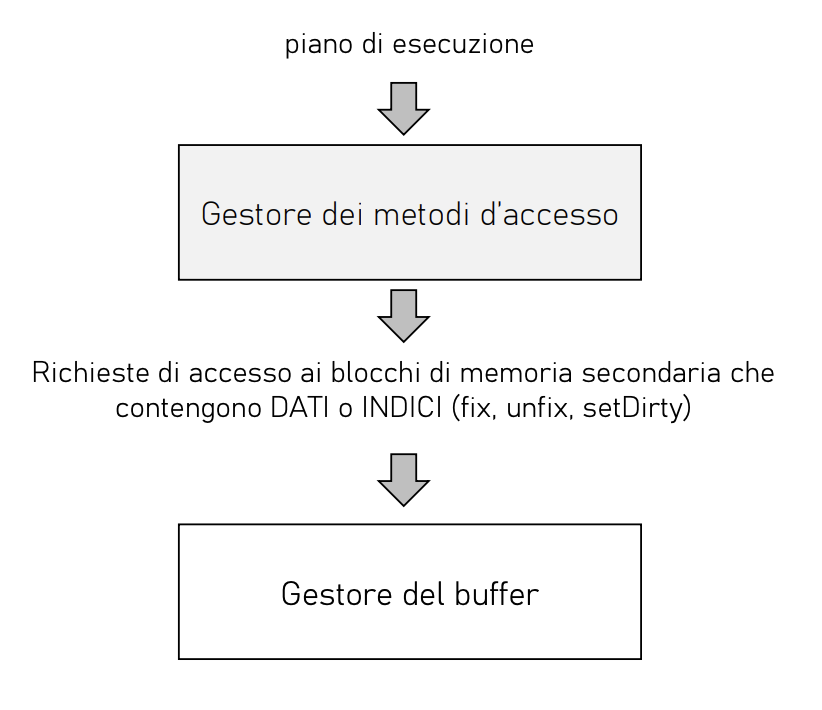
\includegraphics[width=0.6\textwidth]{images/gestore-accesso.png}
  \caption{gestore dei meotodi di accesso}
\end{figure}

\subsection{Metodi di accesso}
I metodi di accesso sono moduli software (es. scansione sequenziale, accesso via indice, ordinamento, varie implementazioni del join) che implementano gli algoritmi di accesso e manipolazione dei dati organizzati in specifiche strutture fisiche.

Ogni metodo di accesso conosce:
\begin{itemize}[label=$\diamond$]
  \item \textbf{organizzazione in tuple} (o dei record di indice) nei blocchi dati (indice) salavati in memoria secondaria
  \smallskip
  \item \textbf{organizzazione fisica interna delle pagine} sia quando contengono dati, sia quando contengono strutture fisiche di accesso (indici)
\end{itemize}

\subsection{Organizzazione di una pagina}
All'interno di una pagina sono presenti:
\begin{itemize}[label=$\triangleright$]
  \item \textbf{informazioni utili}: dati veri e propri (tuple della tabella)
  \smallskip
  \item \textbf{informazioni di controllo}: consentono di accedere alle informazioni utili (dizionario, bt di parità, altre informazioni del file system o della specifica struttura fisica)
\end{itemize}

\begin{figure}[H]
  \centering
  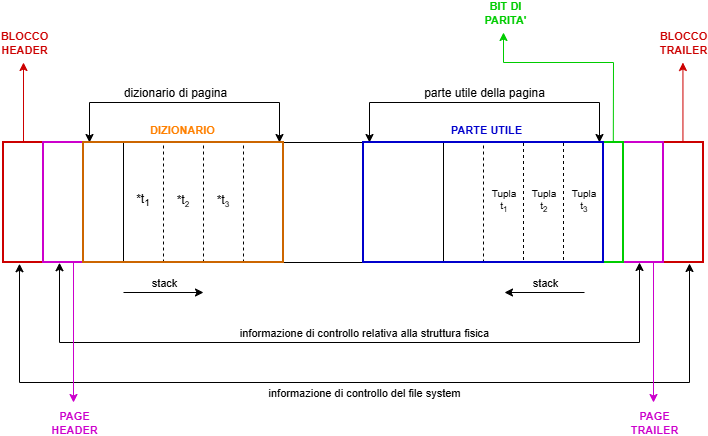
\includegraphics[width=0.6\textwidth]{images/organizzazione-pagina.png}
  \caption{organizzazione di una pagina}
\end{figure}

\begin{itemize}[label=$\Rightarrow$]
  \item \textcolor{red}{\textbf{blocco header/trailer}}: contengono informazioni di controllo utilizzate daò file system
  \smallskip
  \item \textcolor{violet}{\textbf{pagina header/trailer}}: contengono le informazioni di controllo relative alla specifica struttura fisica
  \smallskip
  \item \textcolor{orange}{\textbf{dizionario di pagina}}: contiene i puntatori a ciascun dato utile elementare contenuto nella pagina
  \smallskip
  \item \textcolor{green}{\textbf{bit di parità}}: verifica che l'informazione contenuta nella pagina sia valida
  \smallskip
  \item \textcolor{blue}{\textbf{parte utile}}: contiene i dati
\end{itemize}

\vario{N.B.}{
  Dizionari di pagina e parte utile crescono come stack contrapposti, lasciando libera la parte centrale in uno spazio contiguo.
}

In caso di \textbf{tuple di lunghezza fissa}, il dizionario non è necessario: si memorizza la dimensione delle tutple e l'offset del punto iniziale.\\[0.2ex]
In caso di di \textbf{tuple di lunghezza variabile}, il dizionario memorizza l'offset di ogni tupla presente nel blocco e di ogni attributo di ogni tupla.

Molti gestori delle pagine non consentono la separazione di una tupla su più pagine:
\begin{equation*}
  \text{dimensione massima tupla} = \text{dimensione massima area disponibile su un blocco}
\end{equation*}

Alcuni gestori delle pagine consentono di distribuire una tupla su più pagine, altrimenti va gestito il caso di tuple memorizzato su più pagine.

\subsection{Operazioni sulle pagine}
Le princpali operazioni che si possono eseguire sulle pagine sono:
\begin{itemize}[label=$\triangleright$]
  \item \textbf{inserimento/aggiornamento di una tupla}:
  \begin{itemize}[label=$\diamond$]
    \item esiste spazio contiguo sufficiente: Inserimento
    \smallskip
    \item non esiste spazio contiguo sufficiente, ma spazio sufficiente: riorganizzazione dello spazio + inserimento
    \smallskip
    \item non esiste spazio sufficiente: interazione con il file system per allocare nuovi blocchi per il file
  \end{itemize}
  \smallskip
  \item \textbf{cancellazione contenuto della pagina}
  \smallskip
  \item \textbf{accesso a una tupla}: avviene tramite il valore della chiave o l'offset nel dizionario
  \smallskip
  \item \textbf{accesso a un attributo di una tupla}: identificato in base all’offset e alla lunghezza del campo dopo aver identificato la tuplatramite la chiave o il suo offset 
\end{itemize}


\subsection{Strutture primarie per l'organizzazione dei file}
La struttura prmaria di un file stabilisce il criterio di disposizione delle tuple all'interno del file presente in memoria di massa:
\begin{itemize}[label=$\triangleright$]
  \item \textbf{sequenziale}: colloca le tuple in maniera consecutiva sulla base di un criterio specifico (es. ordine di inserimento)
  \smallskip
  \item \textbf{ad accesso clacolato}: colloca le tuple in posizioni determinate sulla base dell'esecuzione di un algoritmo di hash
  \smallskip
  \item \textbf{ad albero}: utilizzate come strutture secondarie (indici)
\end{itemize}

\begin{figure}[H]
  \centering
  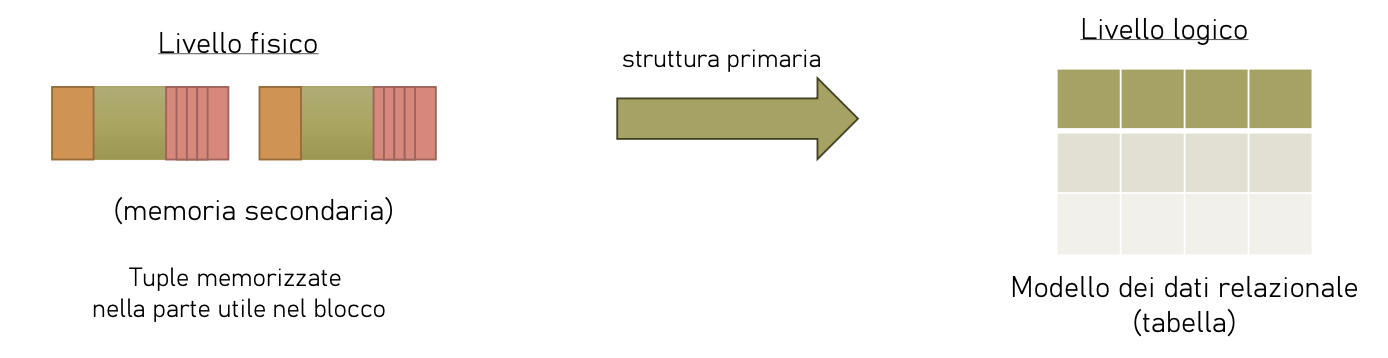
\includegraphics[width=0.6\textwidth]{images/strutture-primarie.png}
  \caption{strutture primarie per l'organizzazione dei file}
\end{figure}

\subsubsection{Struttura sequenziale}
Un file è costituito da blocchi "logicamente" consecutivi e le tuple vengono inserite nei blocchi rispettando una sequenza.

\paragraph{Struttura sequenziale disordinata}
Le tuple sono disposte in
base al loro ordine di inserimento, senza alcun criterio specifico.\\[0.2ex]
Questa è la
struttura più semplice e più diffusa.

\begin{itemize}[label=$\Rightarrow$, itemsep=\smallskipamount]
  \item \textbf{inserimento}:
  \begin{itemize}[label=$\diamond$, itemsep=\smallskipamount]
    \item operazione molto efficiente
    \item sufficiente mantenere uun riferimento all'ultimo blocco
    \item richiede solo un accesso in memoria secondaria
    \item maggiore costo in caso di verifica dei vincoli di integrità
  \end{itemize}
  \item \textbf{ricerca}
  \begin{itemize}[label=$\diamond$, itemsep=\smallskipamount]
    \item operazione non efficiente
    \item richiede ogni volta una scansione sequenziale che consideri tutti i record, con un costo lineare nel numero di blocchi
    \item ricerca può essere fatta usando strutture secondarie (indici)
  \end{itemize}
  \item \textbf{eliminazione}
  \begin{itemize}[label=$\diamond$, itemsep=\smallskipamount]
    \item  facile una volta individuate le tuple coinvolte
    \item si marcano le tuple come "cancellate" senza riorganizzazione locale
  \end{itemize}
  \item \textbf{modifica}
  \begin{itemize}[label=$\diamond$, itemsep=\smallskipamount]
    \item  facile una volta individuate le tuple coinvolte
    \item si procede in loco se possibile, cioè quando non c’è stata nessuna modifica alla dimensione della tupla
    \item si procede con una cancellazione e un inserimento in fondo al file
  \end{itemize}
\end{itemize}

Eliminazioni e modifiche possono portare ad un uso non ottimale dello spazio
siccome si devono effettuare riorganizzazioni periodiche.

\paragraph{Struttura sequenziale ad array}
Le tuple sono disposte come in un array, e la loro posizione dipende dal valore assunto in ciascuna tupla da un campo detto \textbf{indice}.\\[0.2ex]
Questa struttura è utilizzabile soltanto quando le tuple di una tabella
hanno una dimensione fissa, infatti non è quasi masi usata nei DBMS reali perchè difficilmente sono soddisfatte le condizioni per la sua applicazione.

Ad ogni file viene assegnato un numero n di blocchi contigui e ciascun blocco
è dotato di un numero m di posizioni disponibili per le tuple (quindi è un
array bidimensionale n × m).\\[0.2ex]
Ogni tupla è dotata di un valore numerico i
che rappresenta l’indice della tupla in i-esima posizione nell’array.

\begin{itemize}[label=$\Rightarrow$, itemsep=\smallskipamount]
  \item \textbf{inserimento}
  \begin{itemize}[itemsep=\smallskipamount]
    \item Iniziale: l’indice i viene ottenuto incrementando un contatore
    \item Successivo: in una posizione libera oppure alla fine del file
  \end{itemize}
  \item \textbf{cancellazione}: creano delle posizioni libere
\end{itemize}

\paragraph{Struttura sequenziale ordinata}
È un file sequenziale dove le tuple sono ordinate secondo una chiave di ordinamento (diversa dalla chiave primaria).\\[0.2ex]
Questa struttura rende efficienti le operazioni che hanno bisogno
dell’ordinamento utilizzato, ad esempio:
\begin{itemize}[label=$\circ$, itemsep=\smallskipamount]
  \item elenco ordinato
  \item range query
  \item operazioni aggregate
\end{itemize}

In caso di aggiornamento è necessario mantenere l’ordinamento, quindi servono periodiche riorganizzazioni.

\begin{itemize}[label=$\Rightarrow$, itemsep=\smallskipamount]
  \item \textbf{inserimento}
  \begin{enumerate}[itemsep=\smallskipamount]
    \item individuare il blocco B che contiene la tupla che precede, nell’ordine della chiave, la tupla da inserire
    \item se B contiene spazio sufficiente per la nuova tupla allora si inserisce la tupla in B
    \item altrimenti si aggiunge un nuovo blocco, detto overflow page, alla struttura e si inserisce la tupla nel nuovo blocco e si aggiusta la catena di puntatori
  \end{enumerate}
  \item \textbf{scansione sequenziale ordinata secondo la chiave}:  è sufficiente seguire i puntatori
  \item \textbf{cancellazione di una tupla}
  \begin{enumerate}[itemsep=\smallskipamount]
    \item individuare il blocco B che contiene la tupla da cancellare
    \item Cancellare la tupla da B
    \item aggiustare la catena di puntatori
  \end{enumerate}
  \item \textbf{riorganizzazione}: si assegnano le tuple ai blocchi in base ad opportuni coefficienti di riempimento, riaggiustando i puntatori
\end{itemize}

\esempio{struttura sequenziale}{
  Il seguente esempio mostra una struttura sequenziale ordinata secondo la chiave $\texttt{Filiale}$.
  
  \begin{figure}[H]
    \centering
    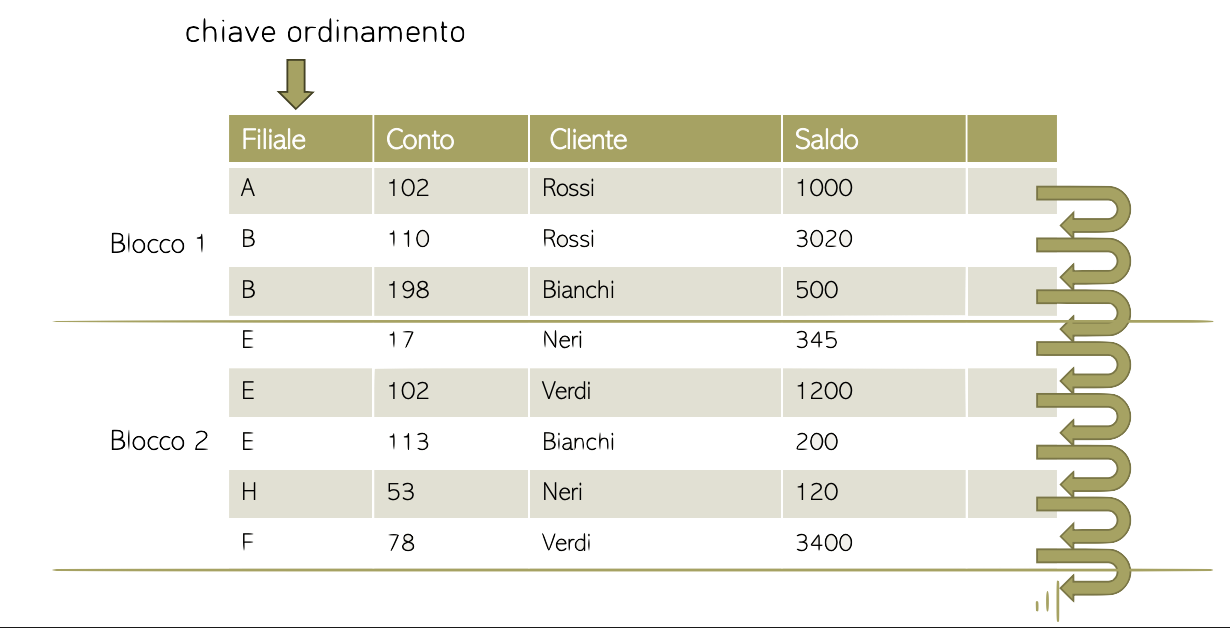
\includegraphics[width=0.6\textwidth]{images/esempio-struttura-sequenziale.png}
  \end{figure}
}

\paragraph{Indice}
Per aumentare le prestazioni degli accessi alle tuple memorizzate nelle strutture fisiche (file sequenziale), si introducono strutture ausiliarie dette strutture di accesso
ai dati, o indici.\\[0.2ex]
Queste strutture velocizzano l’accesso casuale via chiave di ricerca, cioè un insieme di attributi utilizzati nell’indice della ricerca.

Ci sono due tipi di indici su file sequenziali:
\begin{itemize}[label=$\triangleright$, itemsep=\smallskipamount]
  \item \textbf{indice primario}: la chiave di ordinamento del file sequenziale coincide con la chiave di ricerca dell’indice.
  
  Ogni record dell’indice primario contiene una coppia $\langle v_i, p_i\rangle$, dove:
  \begin{itemize}
    \item $v_i$ è il valore della chiave di ricerca
    \item $p_i$ è il puntatore al primo record nel file sequenziale con chiave $v_i$
  \end{itemize}

  Esistono due varianti dell’indice primario:
  \begin{itemize}[itemsep=\smallskipamount]
    \item \textbf{indice denso}: per ogni occorrenza della chiave presente nel file esiste un corrispondente record nell’indice
    \item \textbf{indice sparso}: solo per alcune occorrenze della chiave presenti nel file esiste un corrispondente record nell’indice, tipicamente una per blocco
  \end{itemize}

  Le operazioni che si possono eseguire su un indice primario sono:
  \begin{itemize}
    \item \textbf{ricerca} di una tupla con chiave di ricerca K
    \begin{itemize}
      \item Se l’indice è denso K è presente nell’indice
      \begin{enumerate}
        \item Scansione sequenziale dell’indice per trovare il record (K, pk)
        \item Accesso al file attraverso il puntatore pk
      \end{enumerate}

      Il costo è 1 accesso indice + 1 accesso blocco dati
      \item Se l’indice è sparso K potrebbe non essere presente nell’indice
      \begin{enumerate}
        \item Scansione sequenziale dell’indice fino al record $(K", pk)$, dove $K"$ è il valore più grande che sia minore o uguale a K
        \item Accesso al file attraverso il puntatore pk e scansione del file (blocco corrente) per trovare le tuple con chiave K
      \end{enumerate}

      Il costo è 1 accesso indice + 1 accesso blocco dati
    \end{itemize}

    \item \textbf{Inserimento} di un record nell’indice. Si effettuano gli stessi passi dell’inserimento in un file sequenziale (3.3.5), solo che nel blocco di memoria secondaria al posto di tuple ci sono record di indice.
    \begin{itemize}
      \item Se l’indice è denso l’inserimento nell’indice avviene solo se la tupla inserita nel file ha un valore di chiave K che non è già presente
      \item Se l’indice è sparso l’inserimento avviene solo quando, per effetto dell’inserimento di una nuova tupla, si aggiunge un blocco dati alla struttura; in tutti gli altri casi l’indice rimane invariato
    \end{itemize}

    Gli indici sono costosi, quindi bisogna fare un compromesso sul numero di indici da mantenere e il numero di attributi ad accesso sequenziale.

    \item  \textbf{Cancellazione} di un record nell’indice. Si effettuano gli stessi passi della cancellazione in un file sequenziale (3.3.5)
    \begin{itemize}
      \item  Se l’indice è denso la cancellazione nell’indice avviene solo se la tupla cancellata nel file è l’ultima tupla con valore di chiave K
      \item Se l’indice è sparso la cancellazione nell’indice avviene solo quando K è presente nell’indice e il corrispondente blocco viene eliminato; altrimenti, se il blocco sopravvive, va sostituito K nel record dell’indice con il primo valore $K"$ presente nel blocco.
    \end{itemize}
  \end{itemize}
  \item \textbf{indice secondario}: La chiave di ordinamento e la chiave di ricerca sono diverse.
  
  Ogni record dell’indice secondario contiene una coppia ⟨vi, pi⟩, dove:
  \begin{itemize}
    \item vi è il valore della chiave di ricerca
    \item pi è il puntatore al bucket di puntatori che individuano nel file sequenziale tutte le tuple con chiave vi
  \end{itemize}

  Gli indici secondari sono sempre densi perchè non si può sfruttare l’ordinamento delle tuple.

  Le operazioni che si possono eseguire su un indice secondario sono:
  \begin{itemize}
    \item Ricerca di una tupla con chiave di ricerca K
    \begin{itemize}
      \item Scansione sequenziale dell’indice per trovare il record (K, pk)
      \item Accesso al bucket B di puntatori attraverso il puntatore pk
      \item Accesso al file attraverso i puntatori del bucket B
    \end{itemize}
    
    Il costo è 1 accesso indice + 1 accesso al bucket + n accessi alle pagine dati dove n è il numero di puntatori nel bucket B
    \item  Inserimento e cancellazione: si effettuano gli stessi passi dell’inserimento e della cancellazione in un indice primario denso, con in più l’aggiornamento dei bucket.
  \end{itemize}
\end{itemize}